% (C) Marc Lijour, 2019 
% Licensed under a Creative Commons License BY-SA
% https://creativecommons.org/licenses/by-sa/2.5/ca/
% Presentation for Entrepreneurs at Denton's organized by the Lozard Institute
% Hands-on Introduction to Blockchain
% Presentation touching upon:
% - What is blockchain
% - Hand-on introduction to “crypto” (digital currency, tokens, wallets)
% - ICO market and opportunities
% - Hands-on creation of your own token (ICO basics)
% - Smart contracts
% - Regulations, Token classification, and STOs
% - Main Blockchain technologies used in the Enterprise market
% - Case studies
% - Q&A
% See https://www.eventbrite.ca/e/how-to-implement-blockchain-technology-in-your-business-tickets-49920546699
% 
\frame{
	\frametitle{The Blockchain Peer Group is brought to you by}
	\begin{figure}
		
\includegraphics[width=6cm]{../../Metamesh-LaTeX_Templates/images/logo-black}
	\end{figure}
	\center\Large
	\vspace{-2em}
	\href{https://www.metameshgroup.com}{www.metameshgroup.com}
	
}

\frame{
	\frametitle{Who am I?}
	\framesubtitle{\url{https://www.linkedin.com/in/marclijour/}}
	\begin{columns}
	\column{0.3\textwidth}
		\begin{figure}
		
\includegraphics[width=2cm]{../pics/logos/colliderx_logo}
		\end{figure}
	\column{0.3\textwidth}
		\begin{figure}
		
\includegraphics[width=3.5cm]{../pics/logos/consensys-logo-v-630x581}
		\end{figure}
	\column{0.3\textwidth}
		\begin{figure}
		
\includegraphics[width=3cm]{../../Metamesh-LaTeX_Templates/images/logo-black}
		\end{figure}
	\end{columns}
}

\frame{
	\frametitle{Team Experience}
	\begin{figure}
		\includegraphics[width=11cm]{../pics/Metamesh/metamesh-team-experience}
	\end{figure}
}

\frame{
	\frametitle{Access these slides}
	\center\Huge 
	\url{https://bit.ly/2Tou0Jy}\\ 
	\vspace{2em}
	{\normalsize 
		or find in the folder \href{https://bit.ly/2XtRJYb}{2019 TechConnex - Blockchain Peer Group} at\\
		\url{https://github.com/marclijour/presentations}
	}
}

% ======================================================================================================
%                         Introduction to the presentation and What is Blockchain 
% ======================================================================================================
\section{What is Blockchain?}
\frame{
	\frametitle{The Trust Machine}
	\begin{figure}
		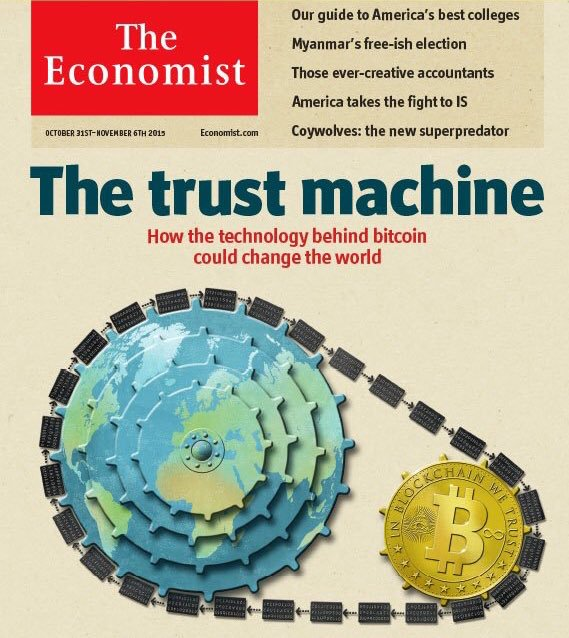
\includegraphics[height=6cm]{../pics/blockchain/economist-trust-machine}
	\end{figure}
}

\frame{
	\frametitle{Source of Trust}
	\framesubtitle{\href{https://www.youtube.com/watch?v=6WG7D47tGb0}{World Economic Forum: \textit{What is Blockchain} Youtube Video}}
	\begin{figure}
		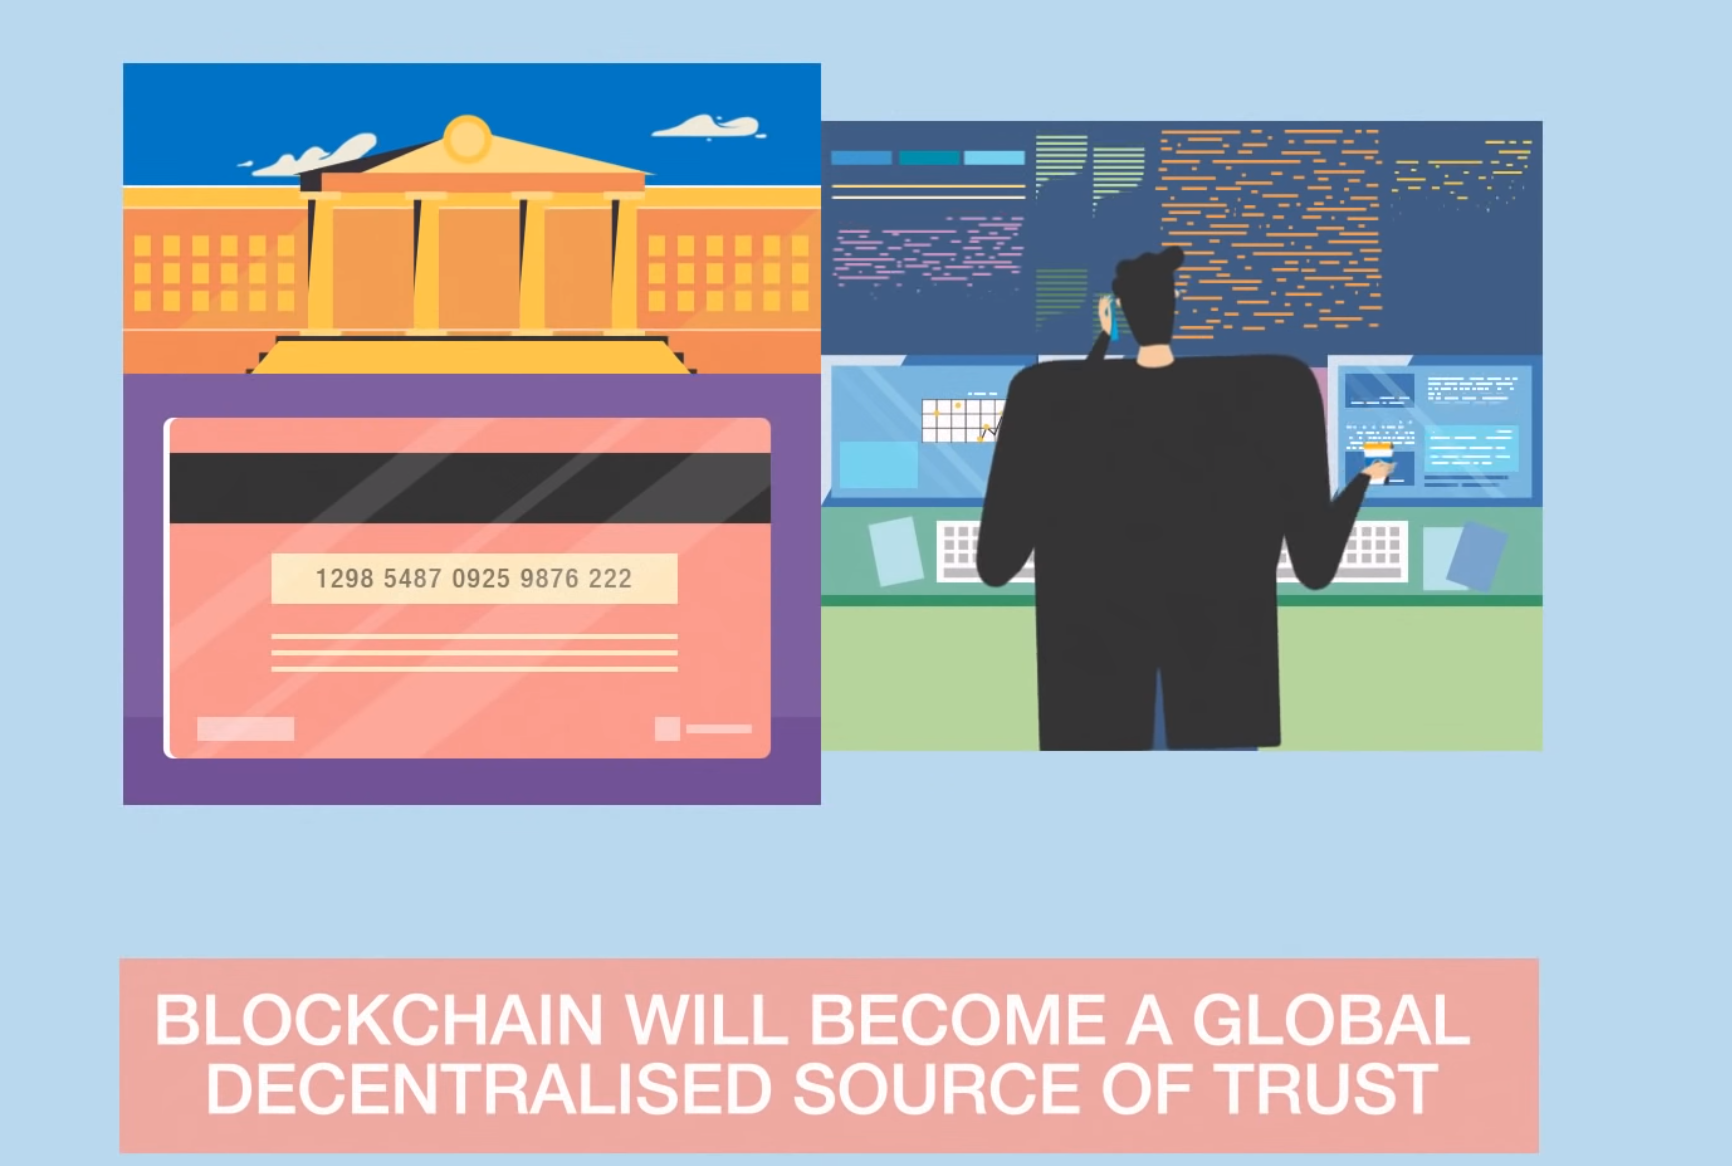
\includegraphics[width=11cm]{../pics/blockchain/wef-blockchain-source-of-trust}
	\end{figure}
}

\frame{
	\frametitle{Key Cryptographic Primitives}
	\begin{columns}[T]
	\column{0.3\textwidth}
		\centering \textbf{Signing}
		\begin{figure}
		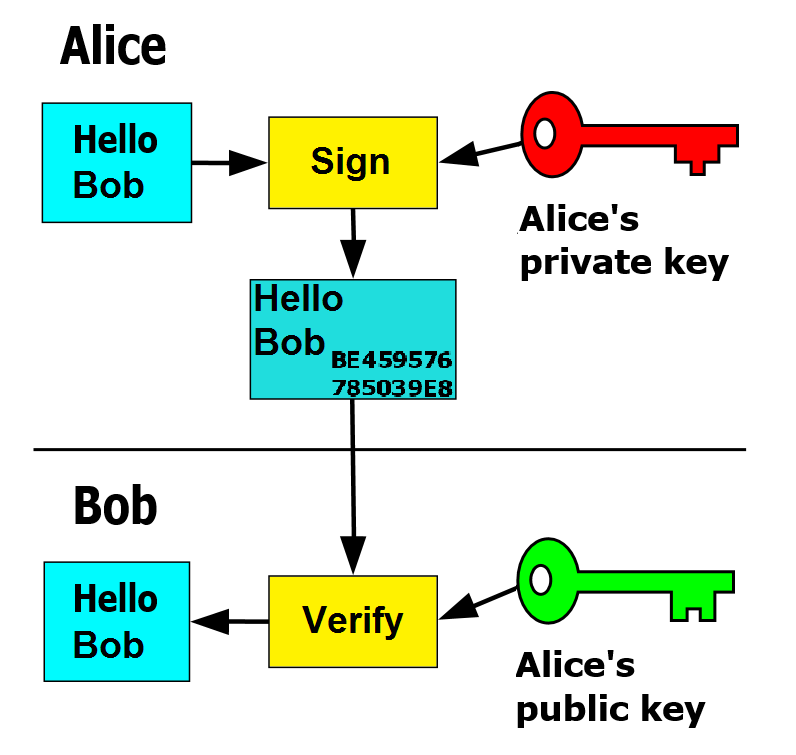
\includegraphics[width=3cm]{../pics/cryptography/Private_key_signing}
		\\
		% CC-BY-SA
		\tiny{Credit: \href{https://commons.wikimedia.org/wiki/User:FlippyFlink}{FlippyFlink}}
		\end{figure}
	\column{0.3\textwidth}
		\centering \textbf{Encrypting}
		\begin{figure}
		% https://en.wikipedia.org/wiki/File:Public_key_encryption.svg
		% public domain
		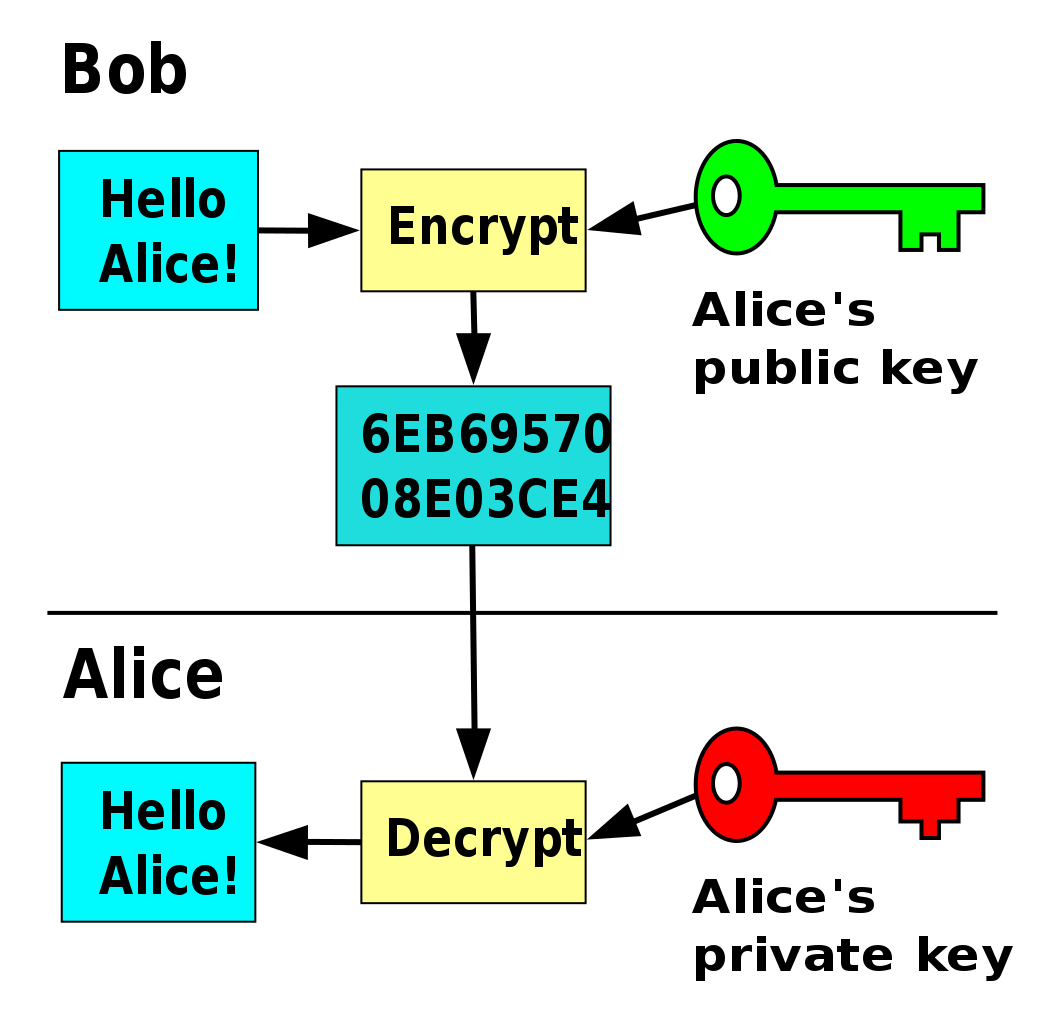
\includegraphics[width=3cm]{../pics/cryptography/1050px-Public_key_encryption}
		\end{figure}
	\column{0.3\textwidth}
		\centering \textbf{Hashing}
		\begin{figure}
		% https://commons.wikimedia.org/wiki/File:Cryptographic_Hash_Function.svg
		% public domain
		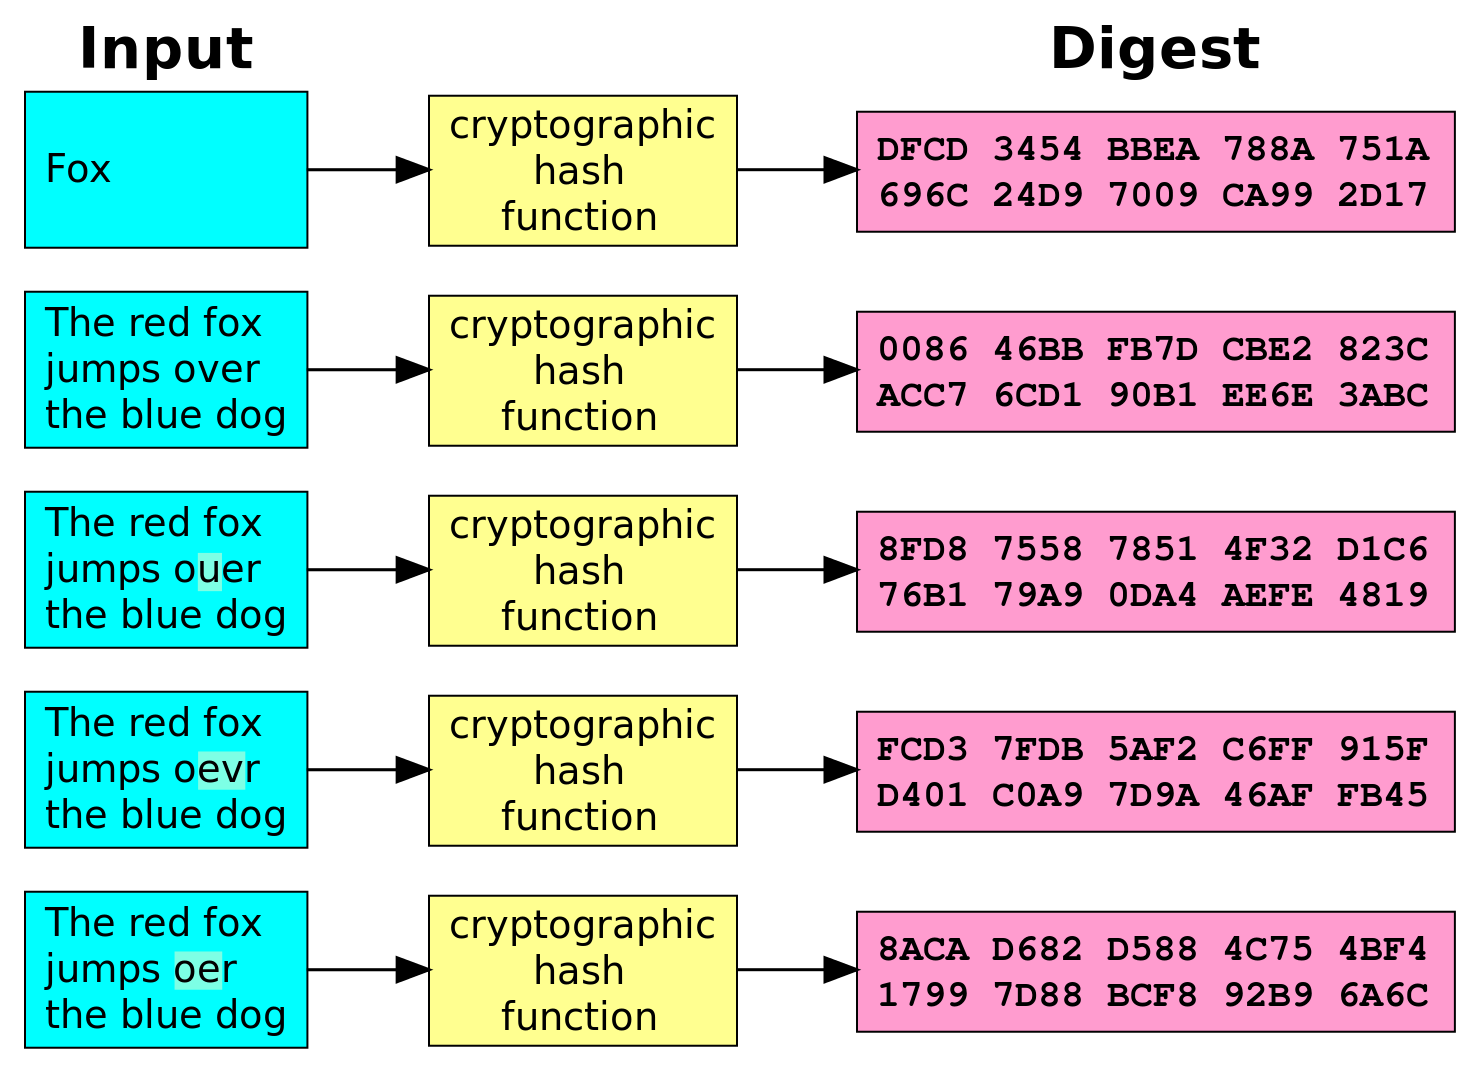
\includegraphics[width=3.6cm]{../pics/cryptography/Cryptographic_Hash_Function}
		\end{figure}
	\end{columns}
}

\frame{
	\frametitle{Where do we need more trust?}
	\begin{itemize}
		\item payments
		\pause
		\item national identity
		\pause
		\item supply chain (e.g. food: \href{https://www.ctvnews.ca/business/france-holds-trial-over-horse-meat-used-in-school-lunches-frozen-lasagna-1.4261868}{Spanghero horse meat trial}, Opioids, expensive cargos)
		\pause
		\item contracts 
		\pause
		\item \textit{real} news \& historical events (e.g. \href{https://media.consensys.net/holding-war-criminals-accountable-with-the-ethereum-blockchain-6b12471a7cdd}{bombings})
		\pause
		\item collaborative data reporting
		\item \ldots
	\end{itemize}
}

% ======================================================================================================
%                         Hands-on Introduction to Crypto, Wallets, and Custom Tokens 
% ======================================================================================================
\section{Hands-on Introduction to Crypto}
\frame{
	\frametitle{}
	\centering\Huge
	Let's try things out!
}

\frame{
	\frametitle{Install MetaMask}
	\begin{columns}
	\column{0.6\textwidth}
		Follow step by step:
		\begin{enumerate}
			\item Install the \href{https://chrome.google.com/webstore/detail/metamask/nkbihfbeogaeaoehlefnkodbefgpgknn}{Chrome/Chromium extension} 
			\item Watch the \href{https://www.youtube.com/watch?v=6Gf\_kRE4MJU}{intro on Youtube}
			\item Create an account 
			\item Switch to the Ropsten Testnet (top-right in MetaMask) 
			\item Fill your account with Ether from \url{https://faucet.metamask.io}
		\end{enumerate}
	\column{0.4\textwidth}
		\begin{figure}
			
\includegraphics[width=3cm]{../pics/ethereum/metamask-logo}
			\captionsetup{justification=centering}
			\caption*{\url{https://metamask.io}}
		\end{figure}
	\end{columns}
}

\frame{
	\frametitle{Request Ether from the faucet (on the Ropsten network)}
	\framesubtitle{Do it several times; then donate 1 ether to the faucet}
	\begin{figure}
		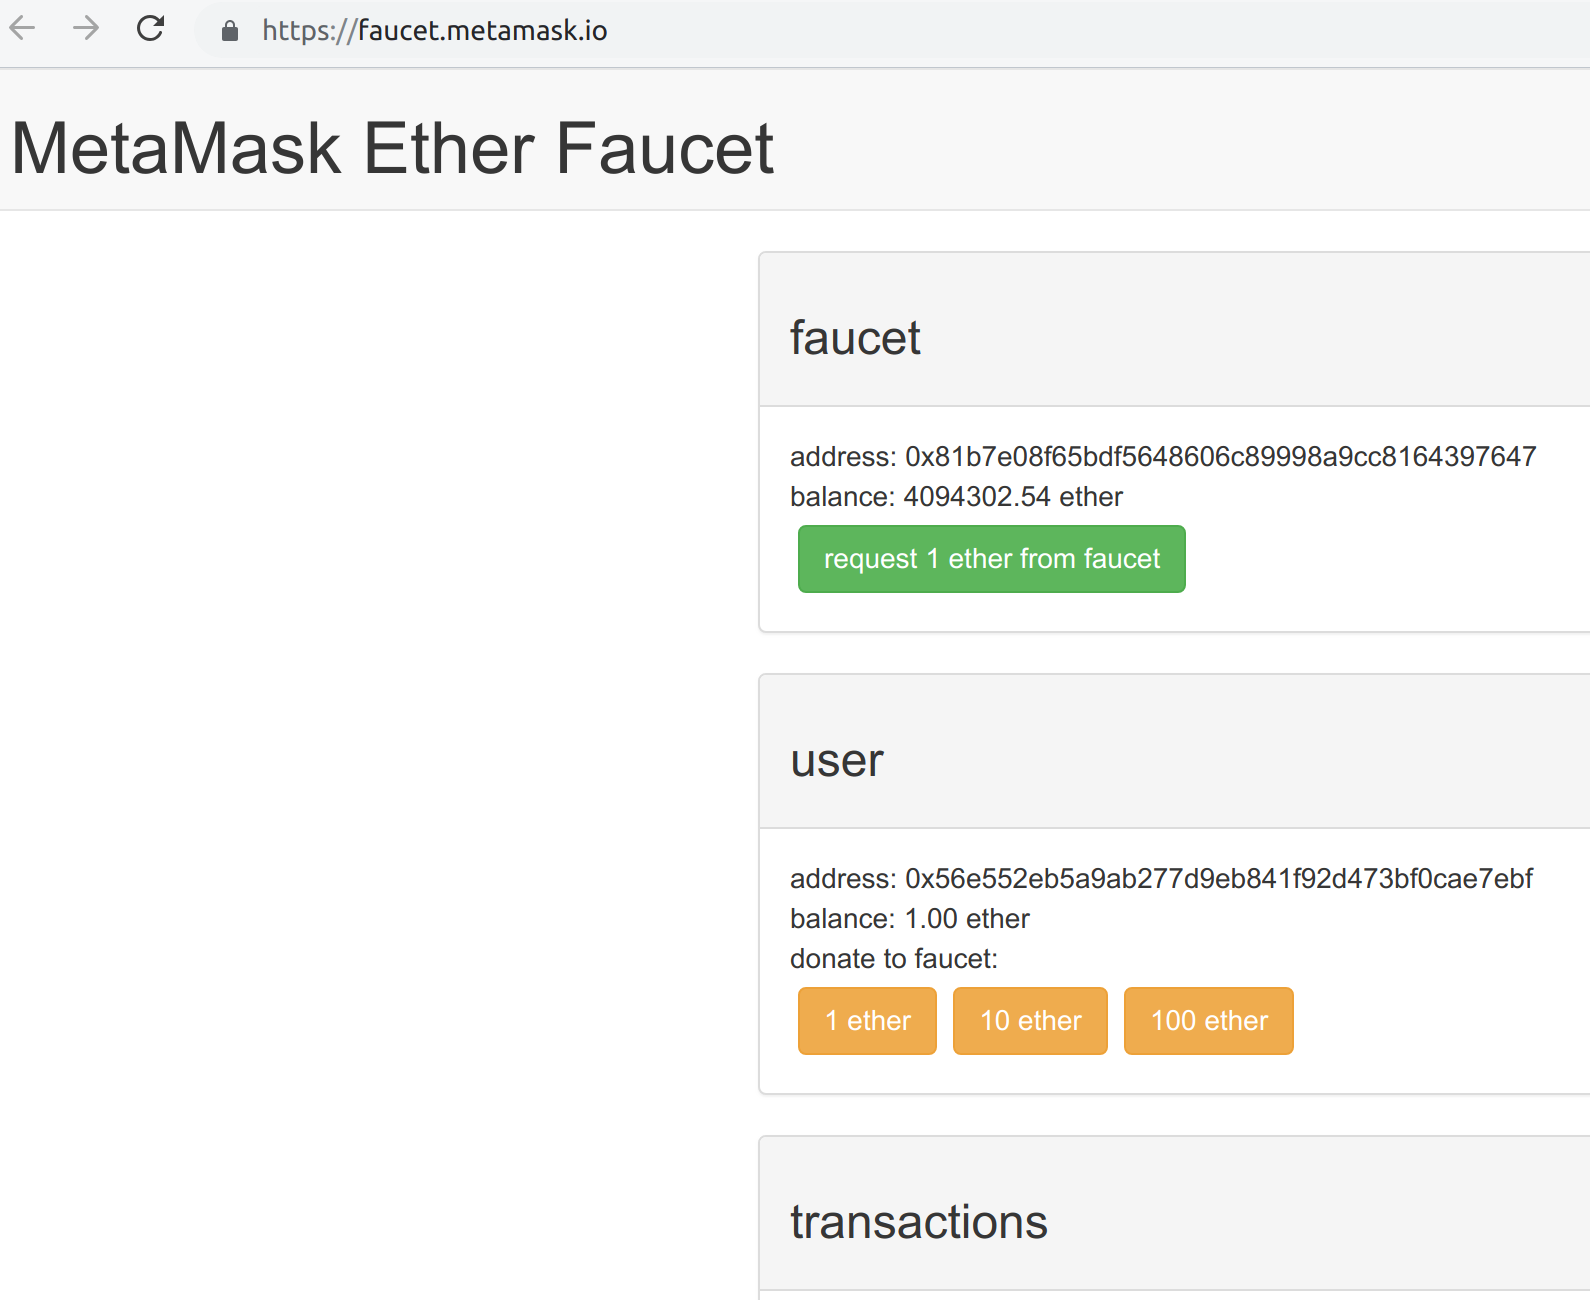
\includegraphics[width=10cm]{../pics/ethereum/faucet-ropsten}
	\end{figure}
}

\frame{
	\frametitle{Check the transaction on Metamask}
	\framesubtitle{Click on the transaction for a detailed view}
	\begin{figure}
		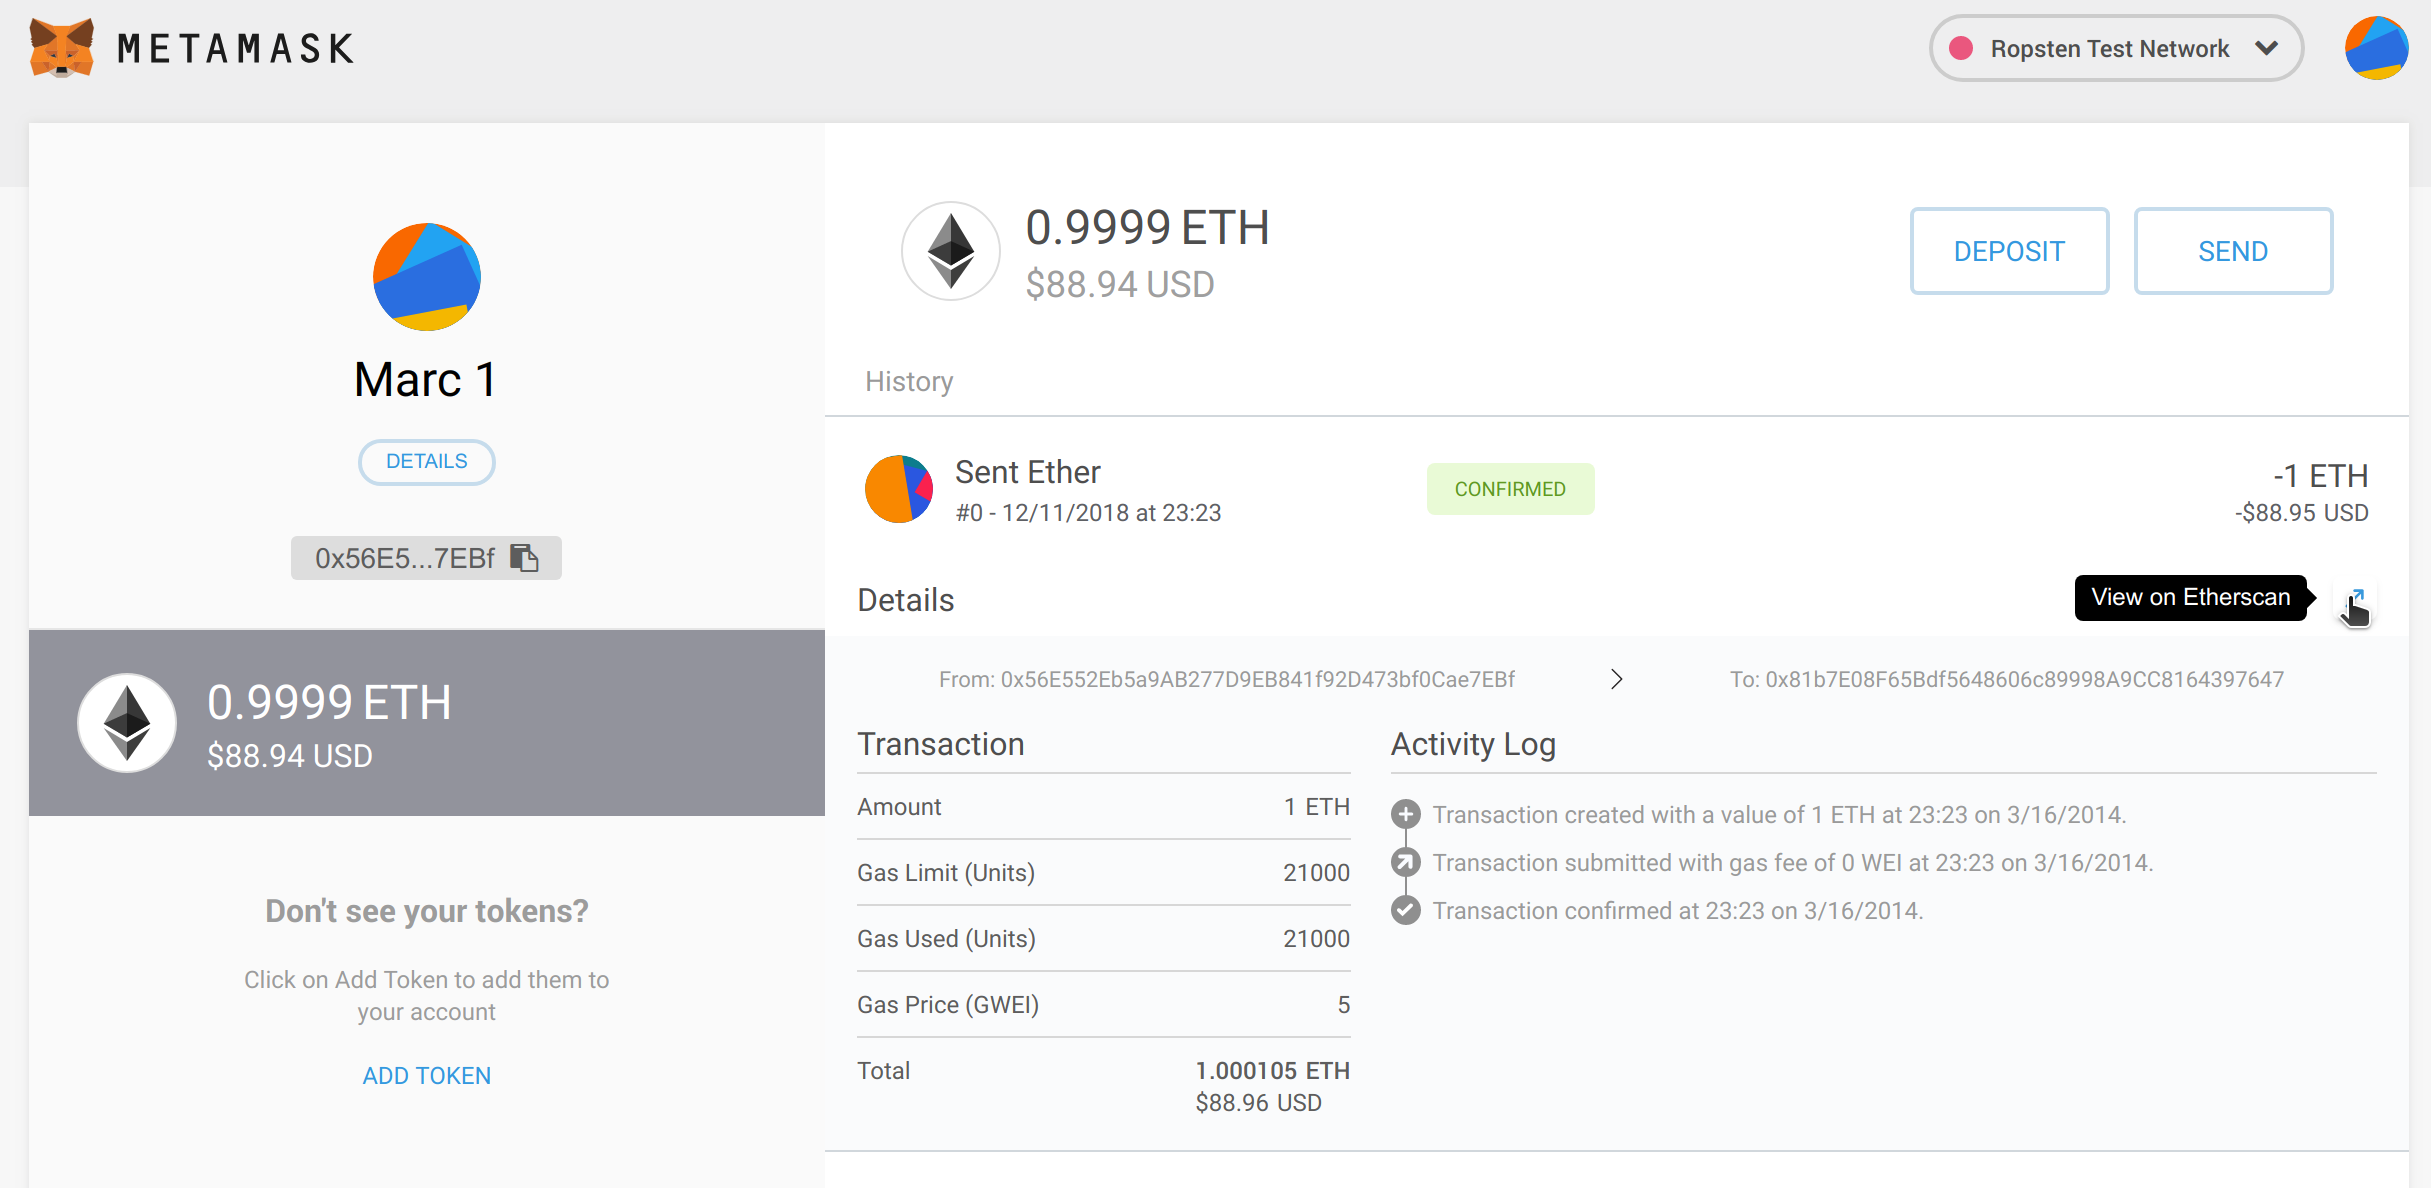
\includegraphics[width=10cm]{../pics/ethereum/metamask-tx-pane-2018}
	\end{figure}
}

\frame{
	\frametitle{Check the transaction on Etherscan}
	\begin{figure}
		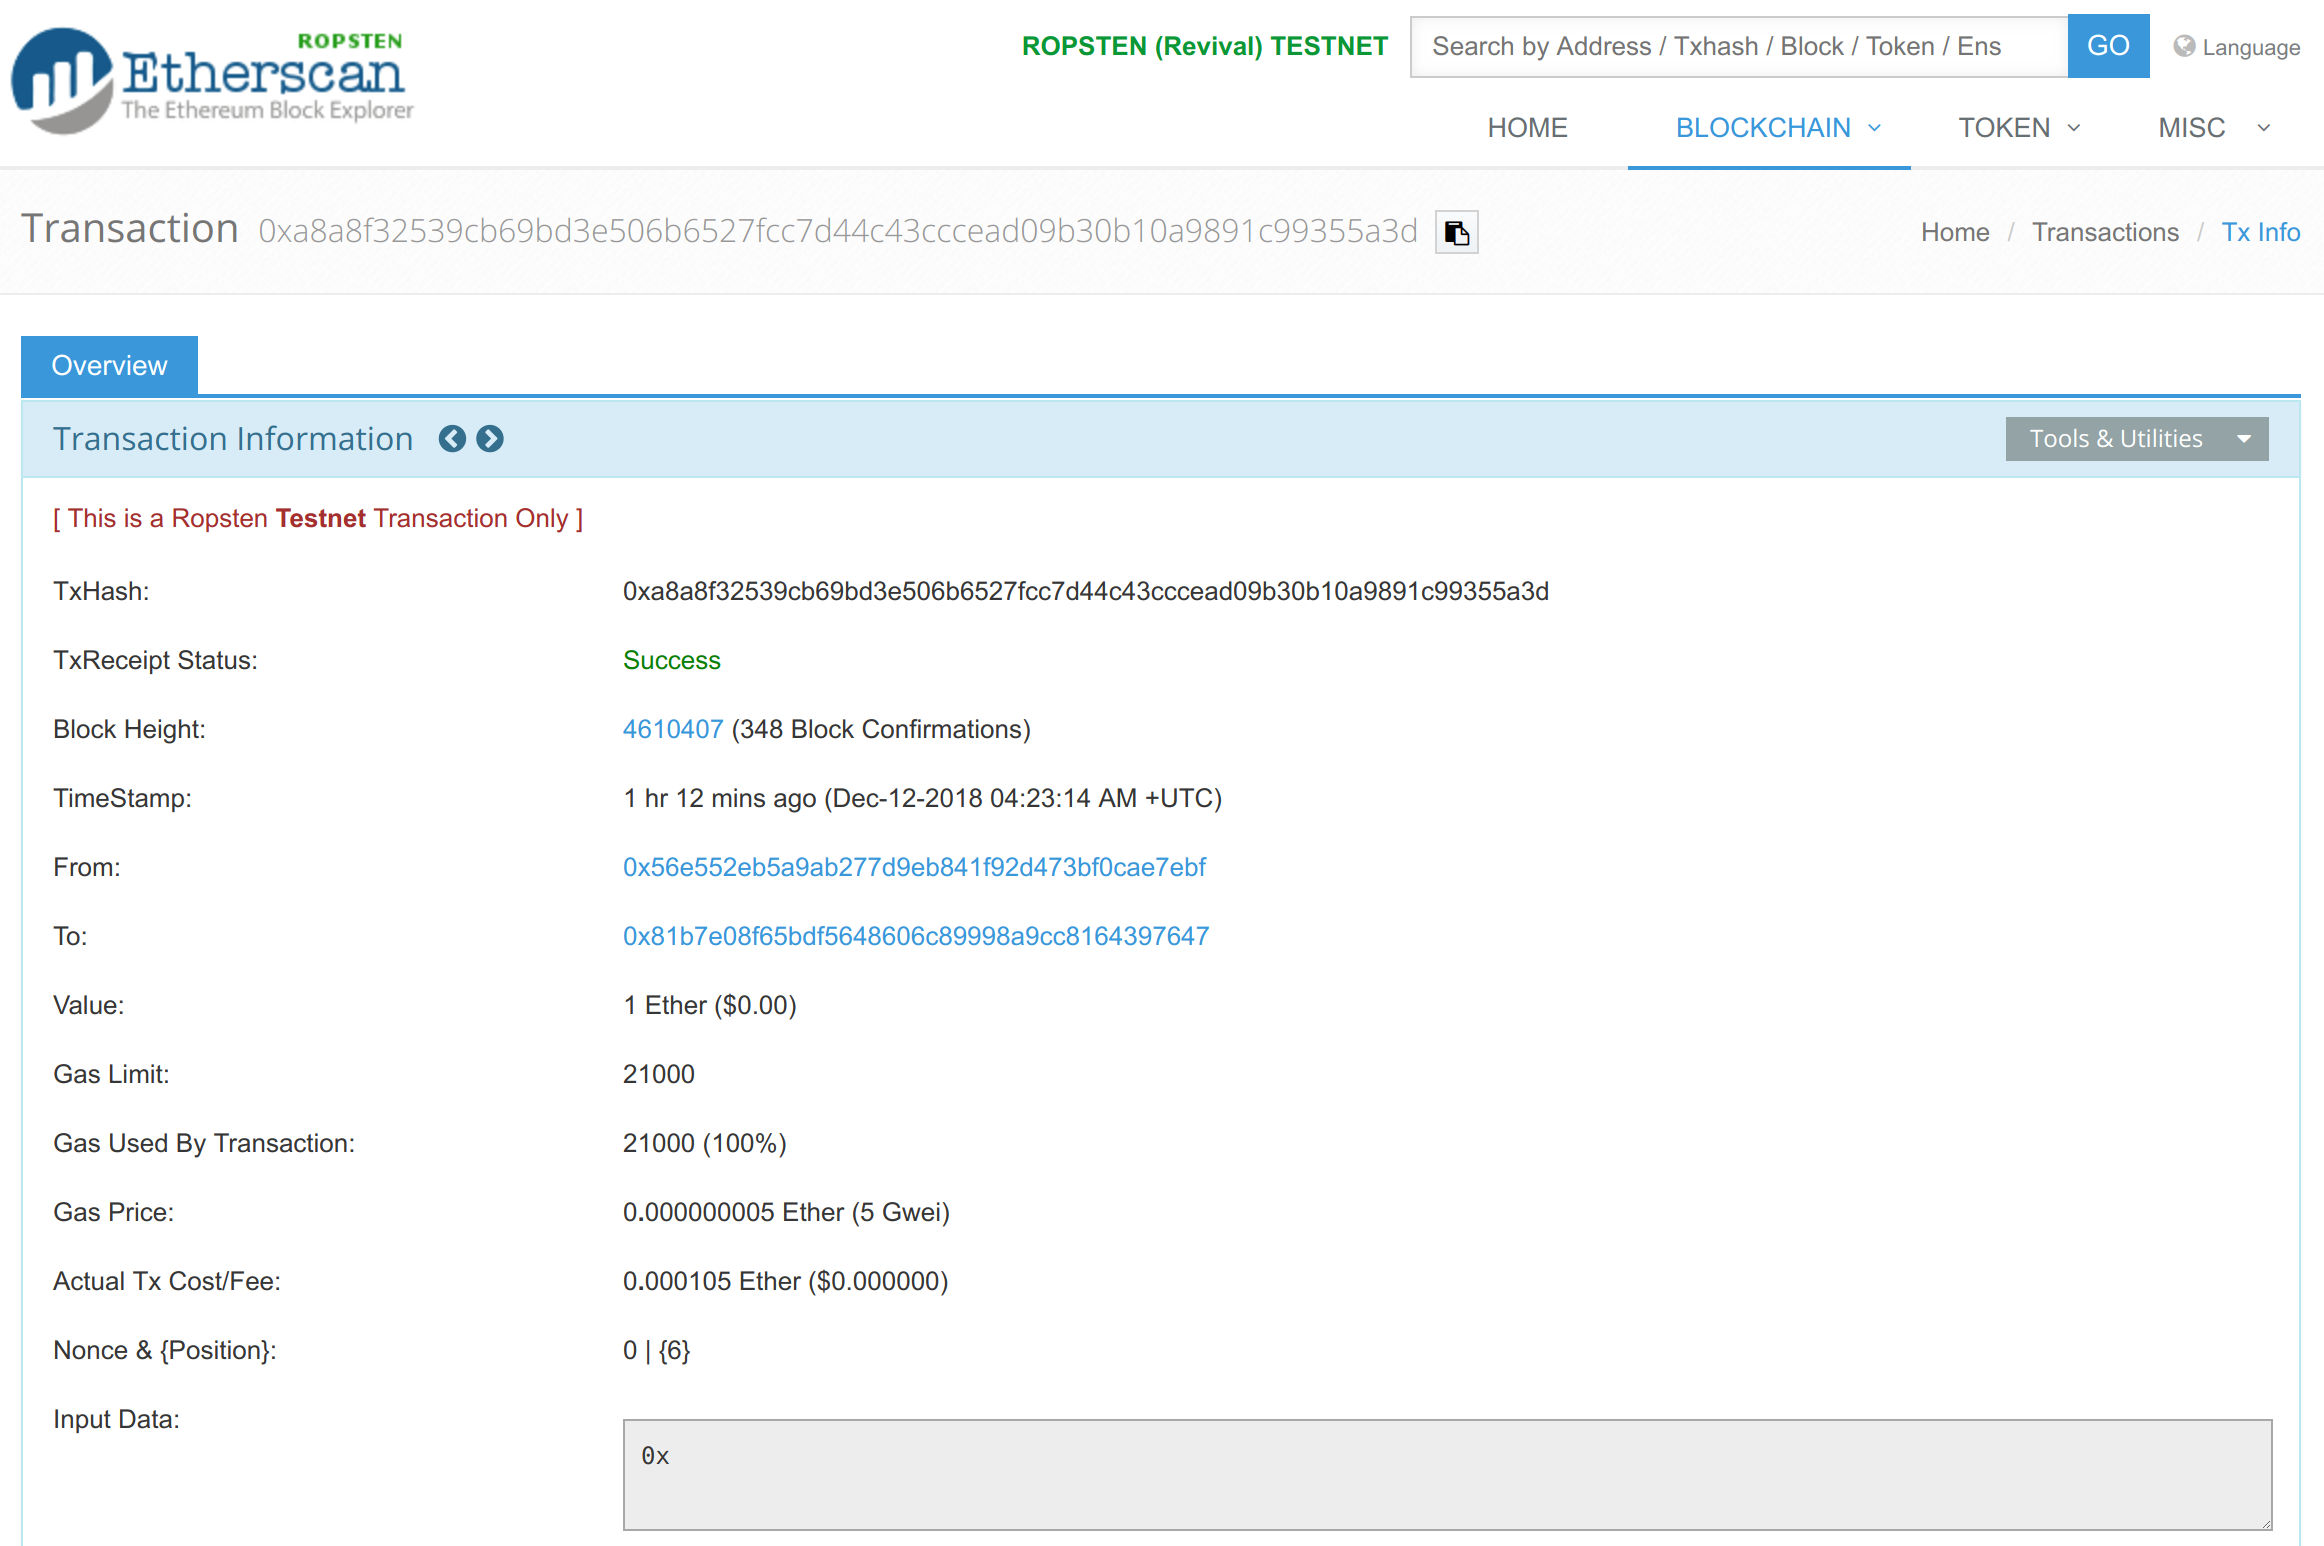
\includegraphics[width=10.9cm]{../pics/ethereum/etherscan-tx-example2}
	\end{figure}
}

\frame{
	\frametitle{A note about gas price}
	\framesubtitle{\url{https://ethgasstation.info}}
	\begin{figure}
		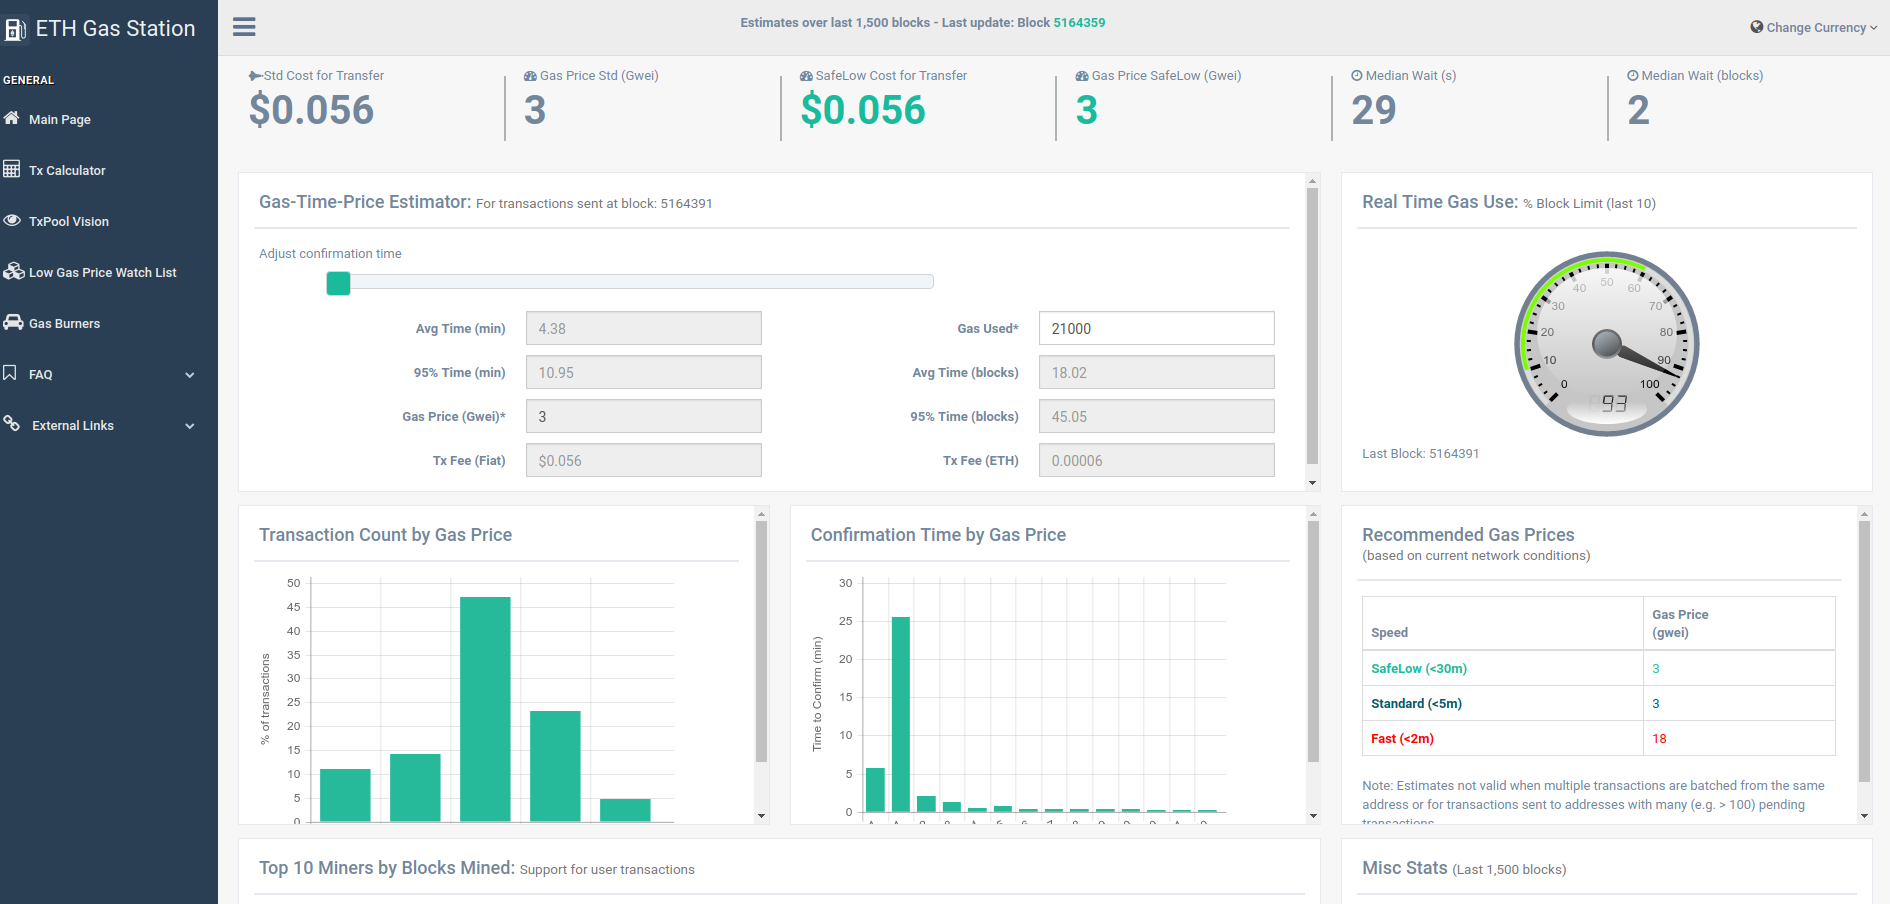
\includegraphics[width=11.5cm]{../pics/ethereum/ethgasstation}
	\end{figure}
}

\frame{
	\frametitle{Price of (real) ether: ETH}
	\framesubtitle{More information: \url{https://www.tradingview.com/symbols/ETHUSD/}}
	\begin{figure}
		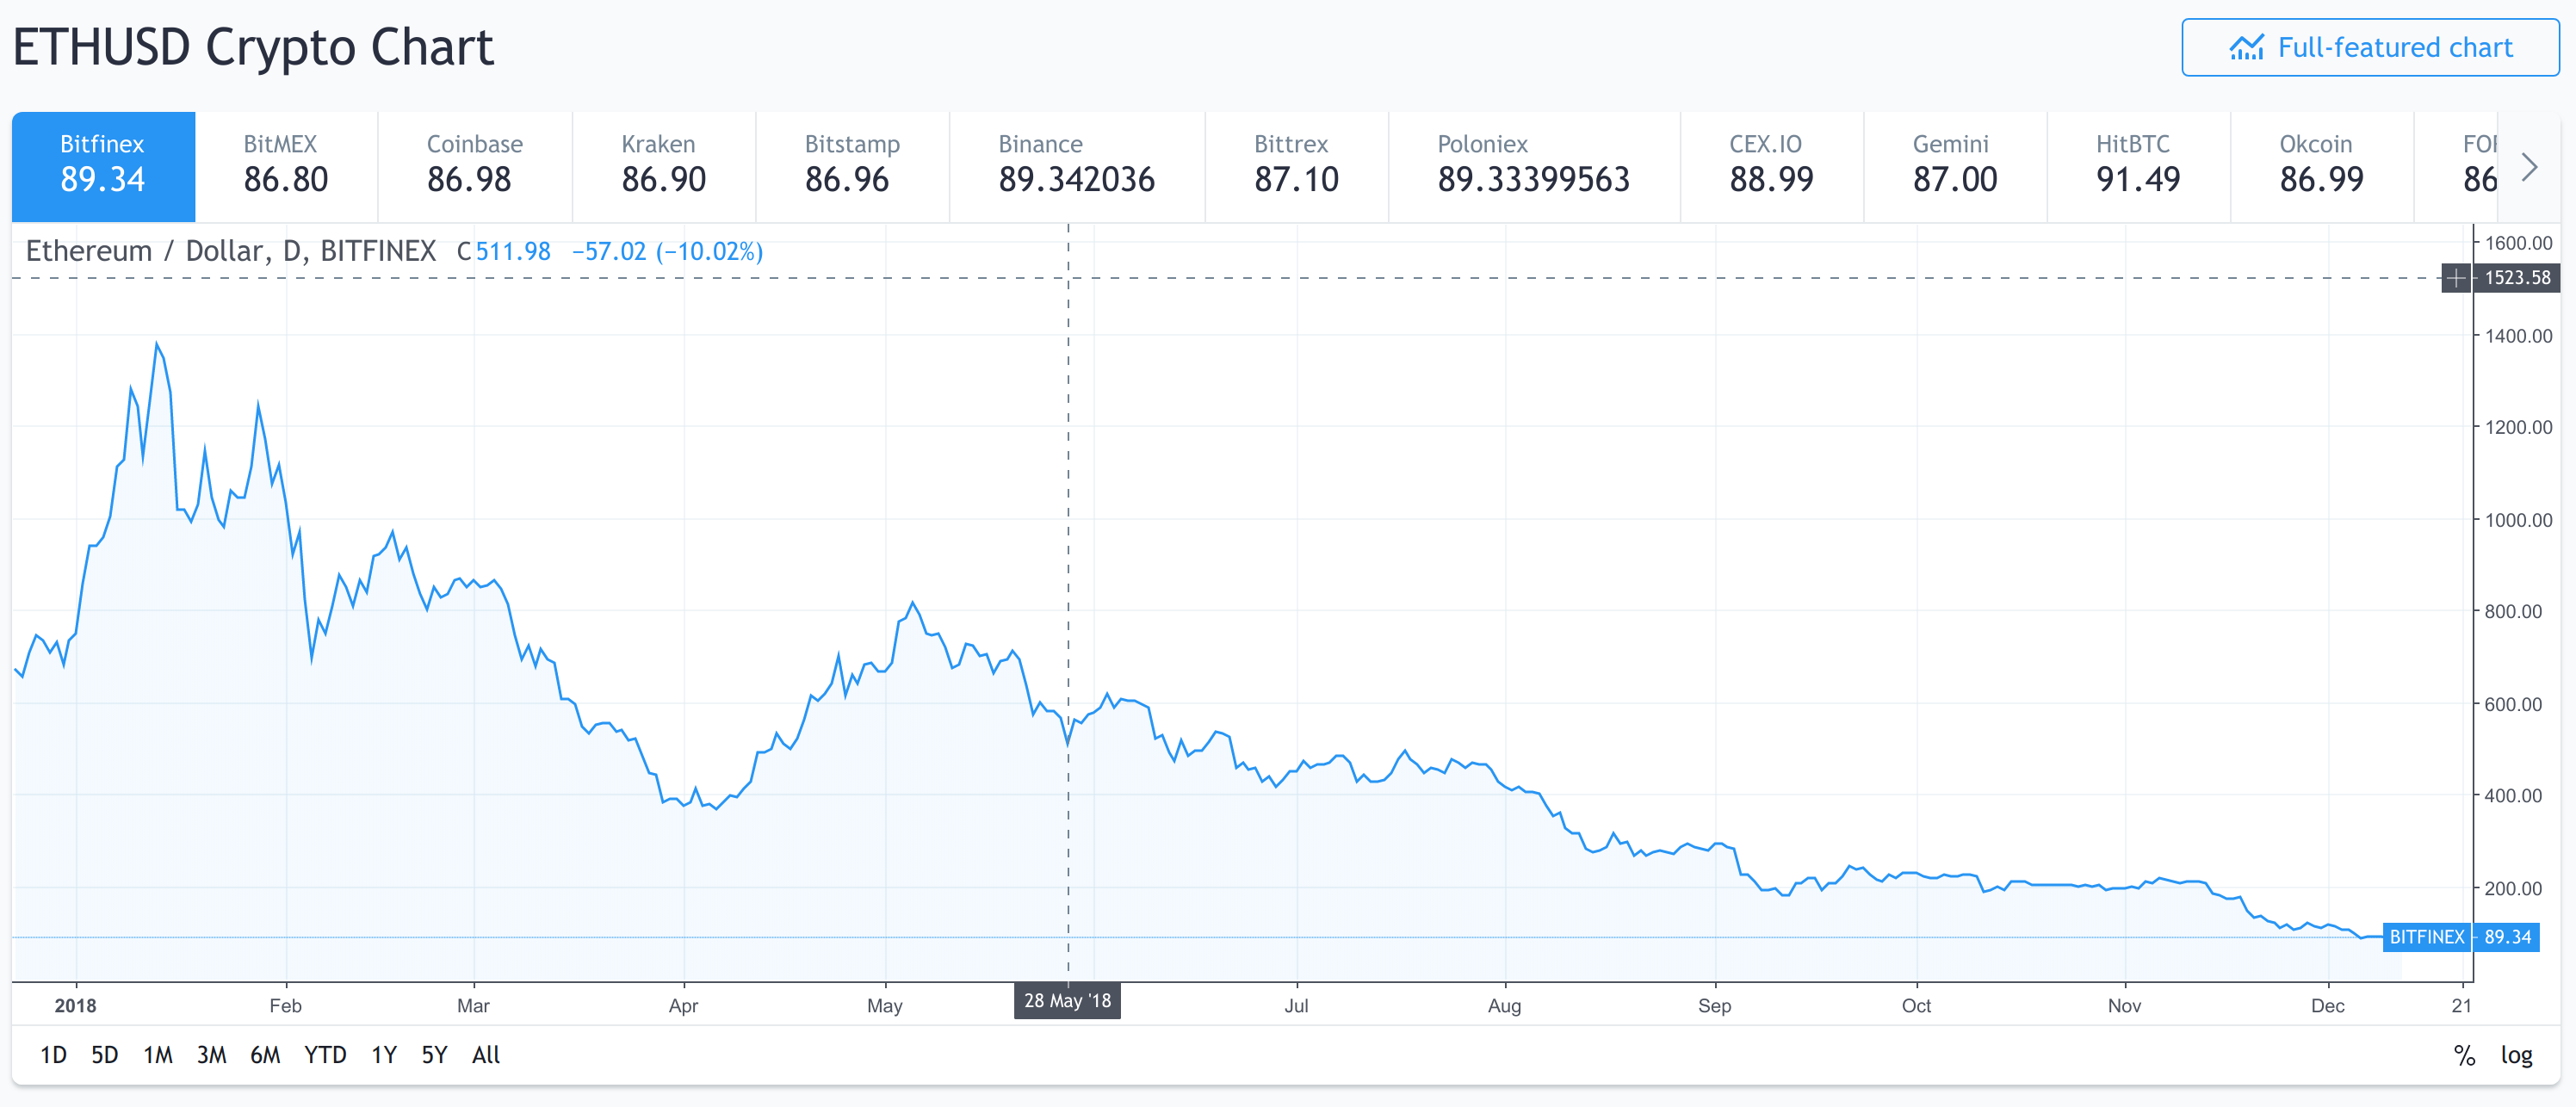
\includegraphics[width=11.5cm]{../pics/ethereum/ETH-USD-2018-12-12}
	\end{figure}
}

\frame{
	\frametitle{Wallets}
	\framesubtitle{More information: \url{https://blockgeeks.com/guides/cryptocurrency-wallet-guide/}}
	\begin{figure}
		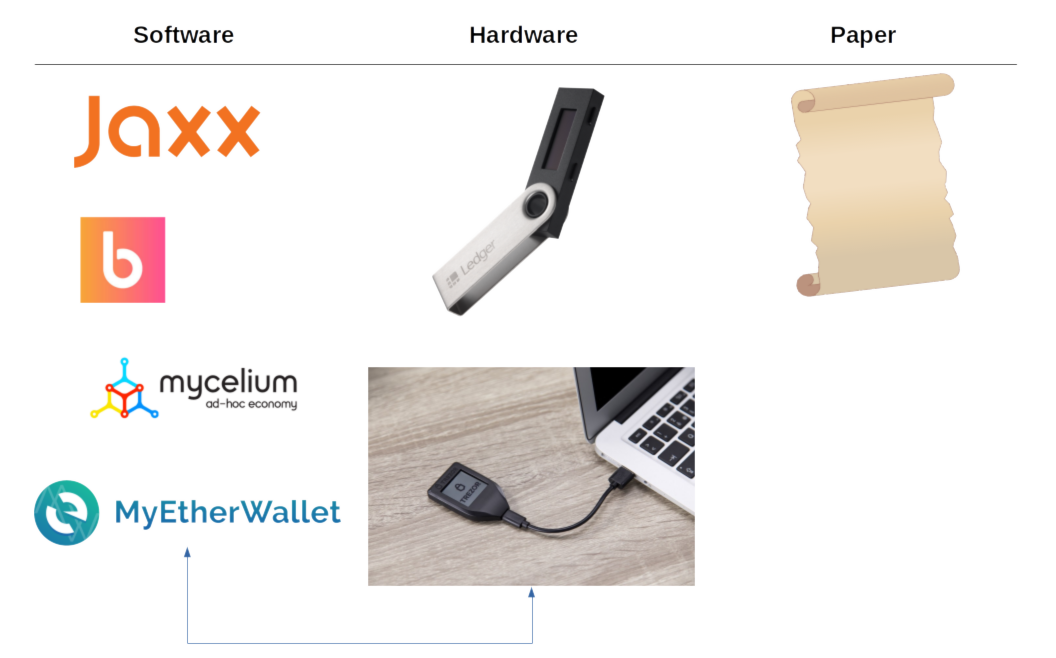
\includegraphics[width=11.5cm]{../pics/ethereum/wallets}
	\end{figure}
}

\frame{
	\frametitle{Exchanges}
	\begin{enumerate}
		\item Centralized Exchanges (Coinbase, Quadriga, ...)
		\item Decentralized Exchanges
	\end{enumerate}
}

\frame{
	\frametitle{ATMs}
	\framesubtitle{More information: \url{https://coinatmradar.com/country/38/bitcoin-atm-canada/}}
	\begin{figure}
		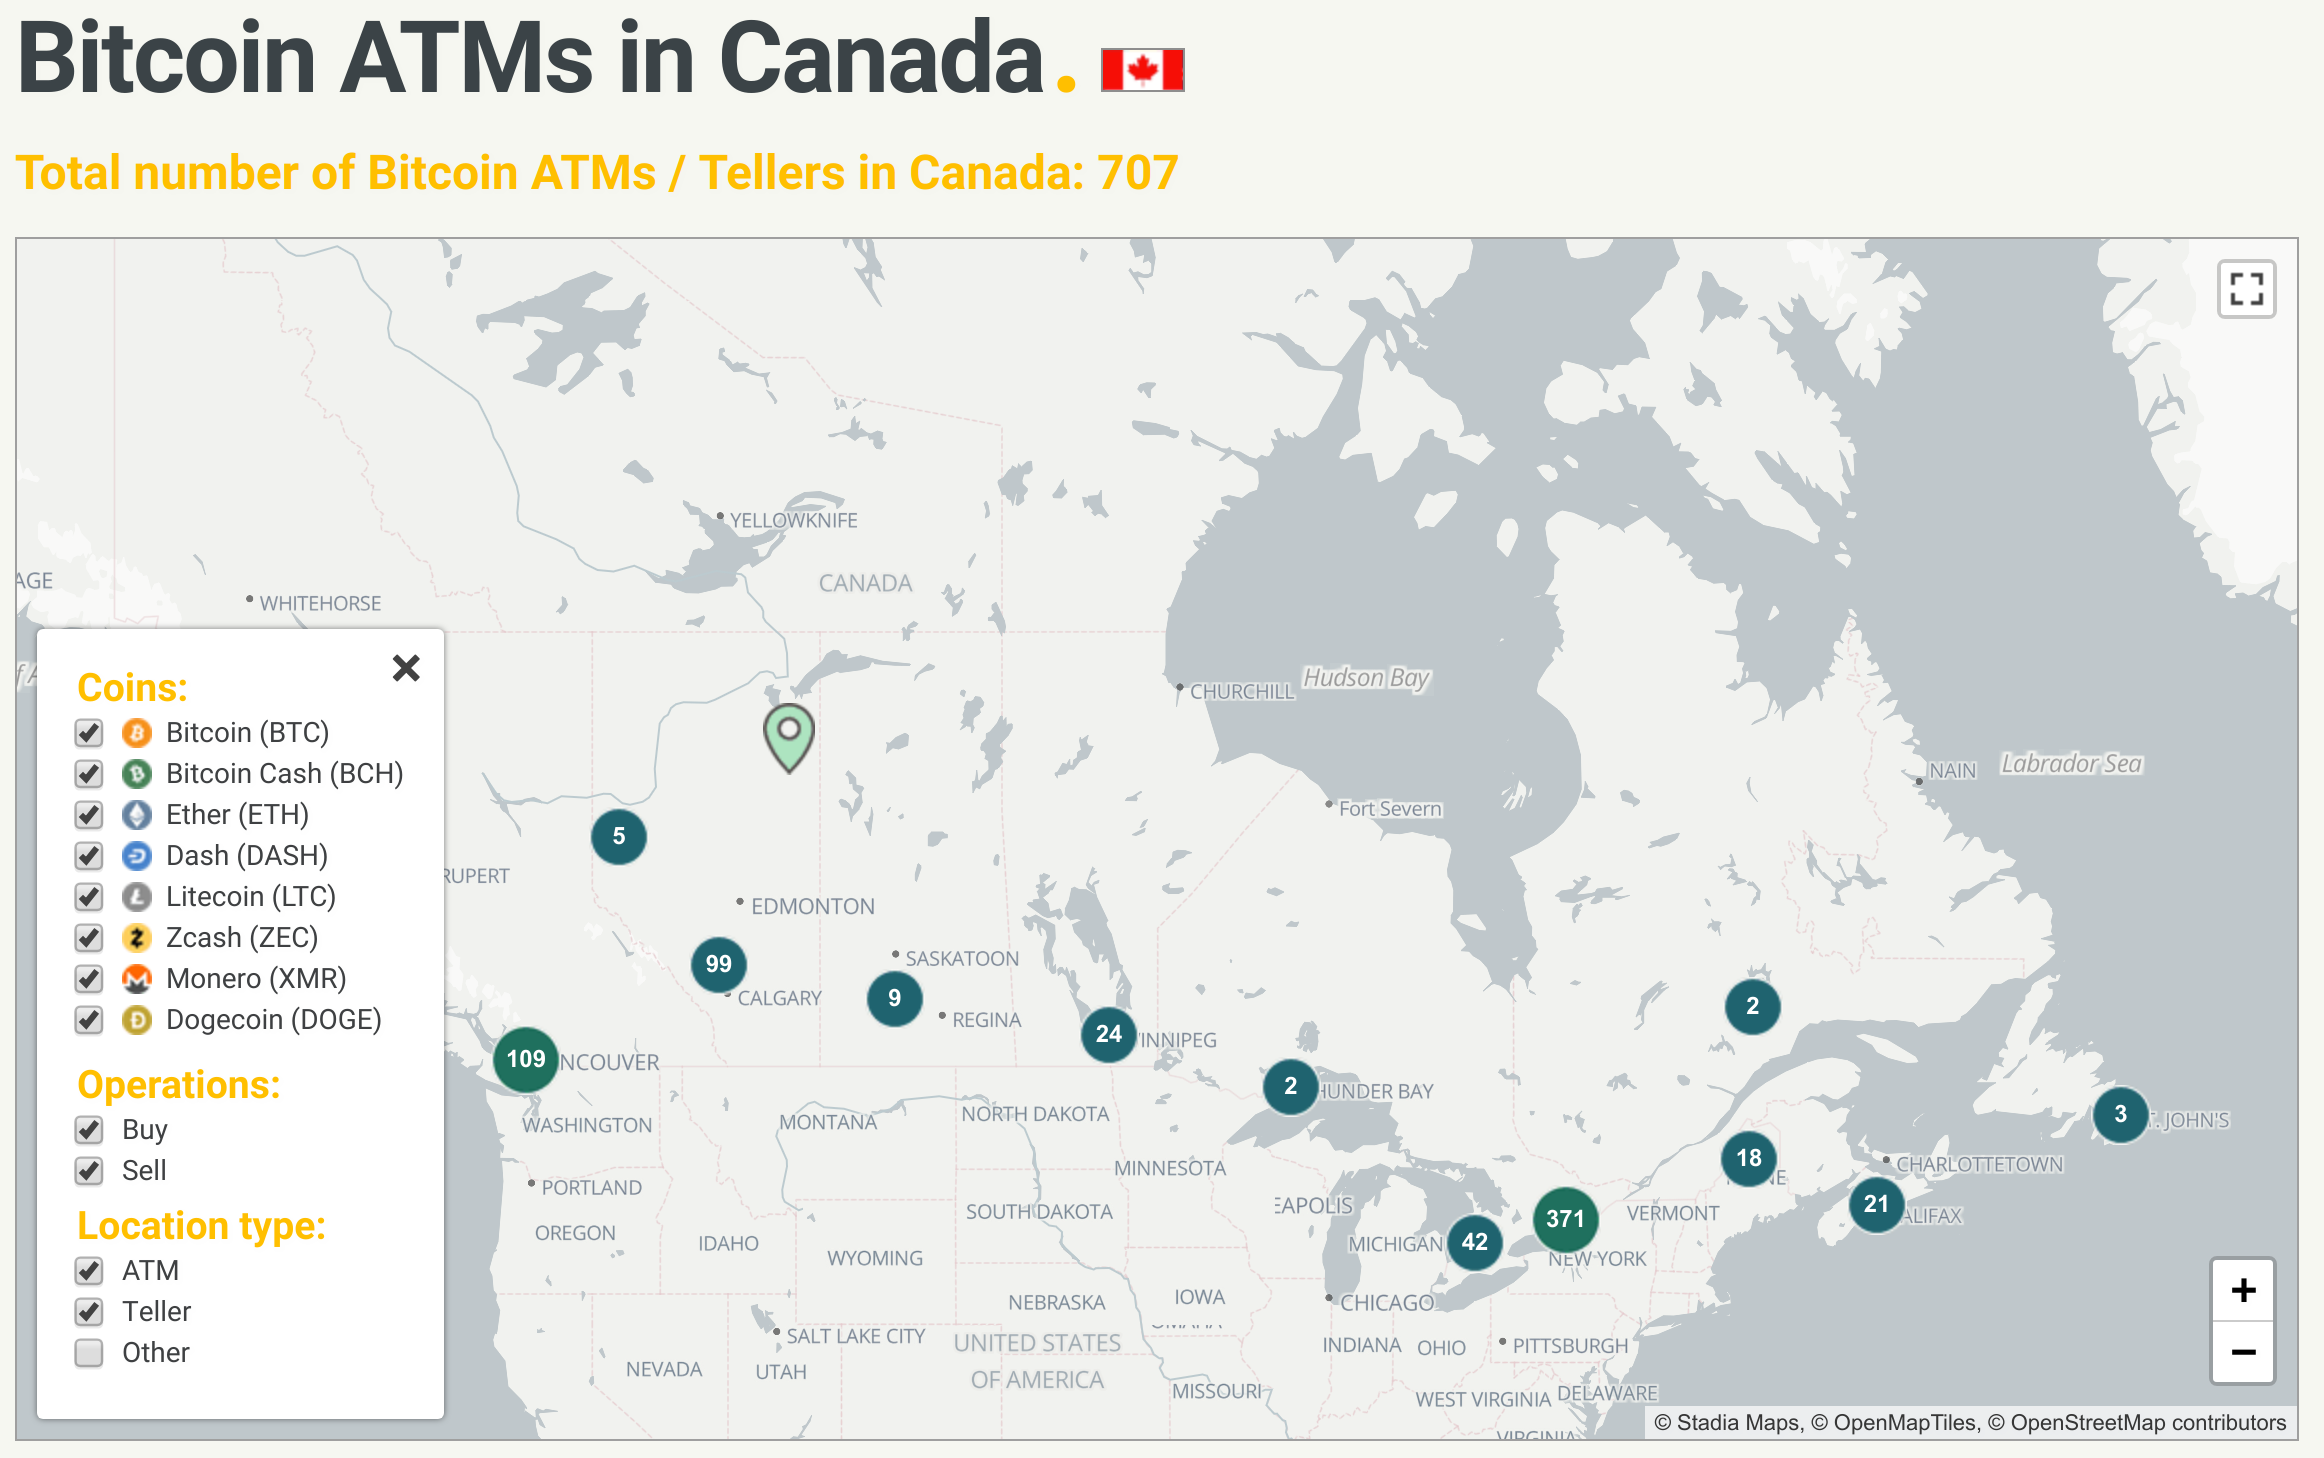
\includegraphics[width=10cm]{../pics/ethereum/bitcoin-atms-canada-2019-01}
	\end{figure}
}

\frame{
	\frametitle{ATMs}
	\framesubtitle{More information: \url{https://coinatmradar.com/country/38/bitcoin-atm-canada/}}
	\begin{figure}
		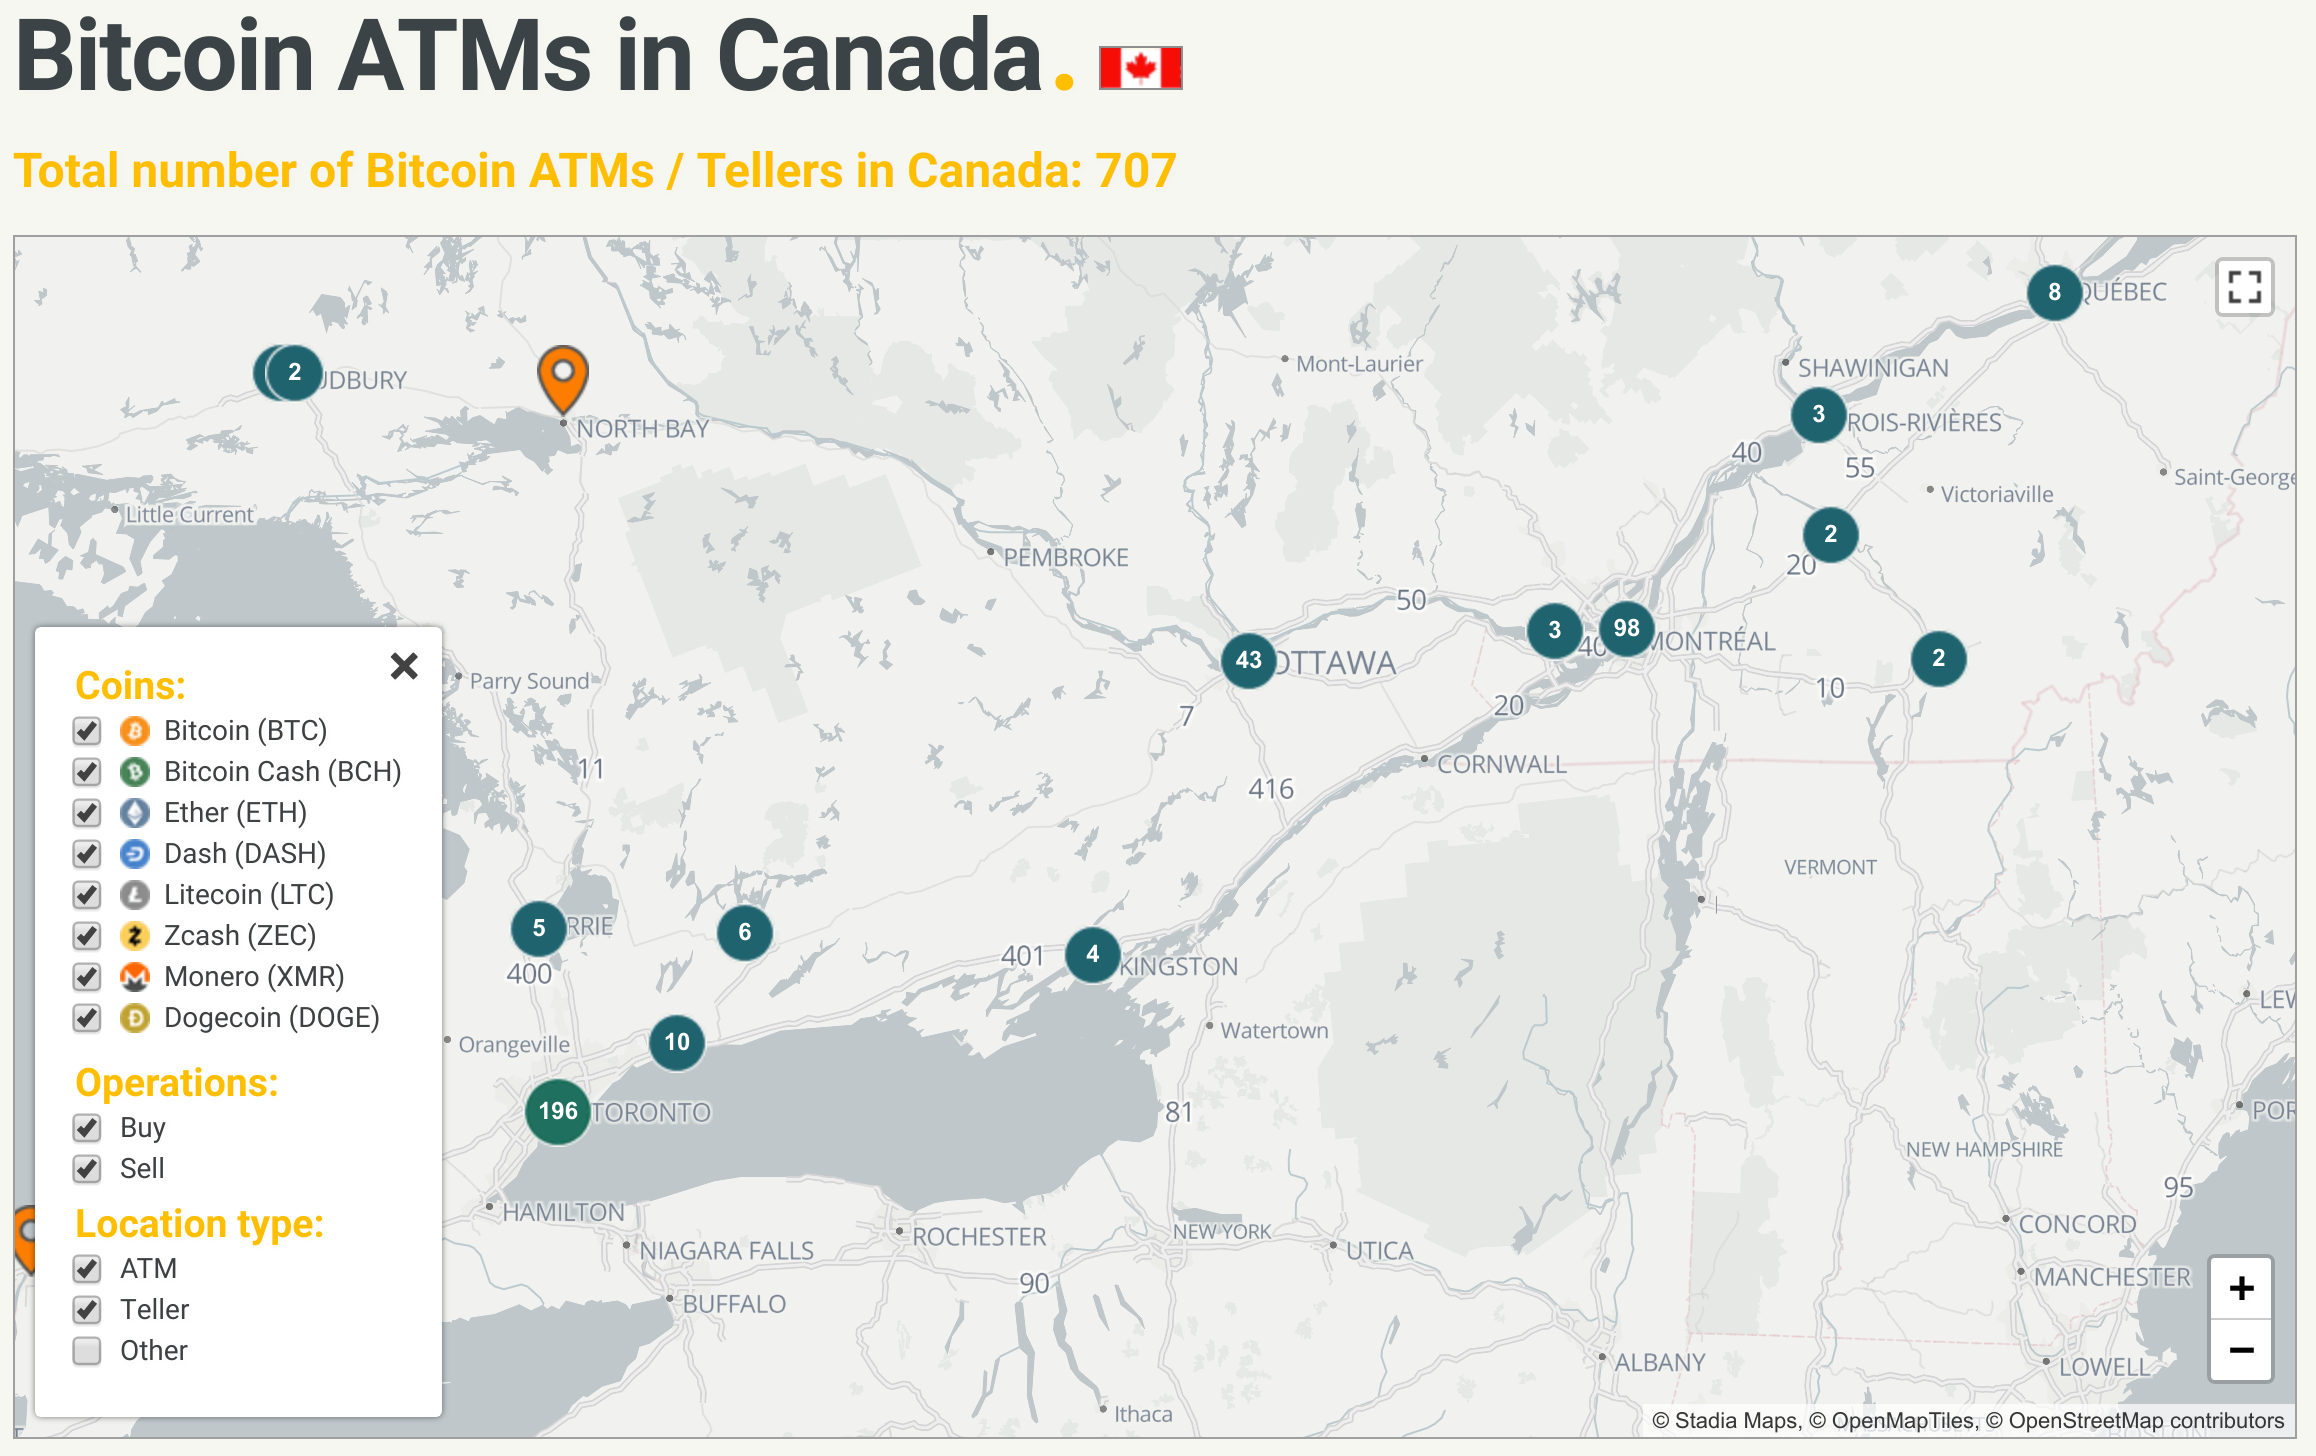
\includegraphics[width=10cm]{../pics/ethereum/bitcoin-atms-ontario-quebec-2019-01}
	\end{figure}
}

\frame{
	\frametitle{Other crypto-assets}
	\framesubtitle{More information: \url{https://www.tradingview.com/markets/cryptocurrencies/prices-all/}}
	\begin{figure}
		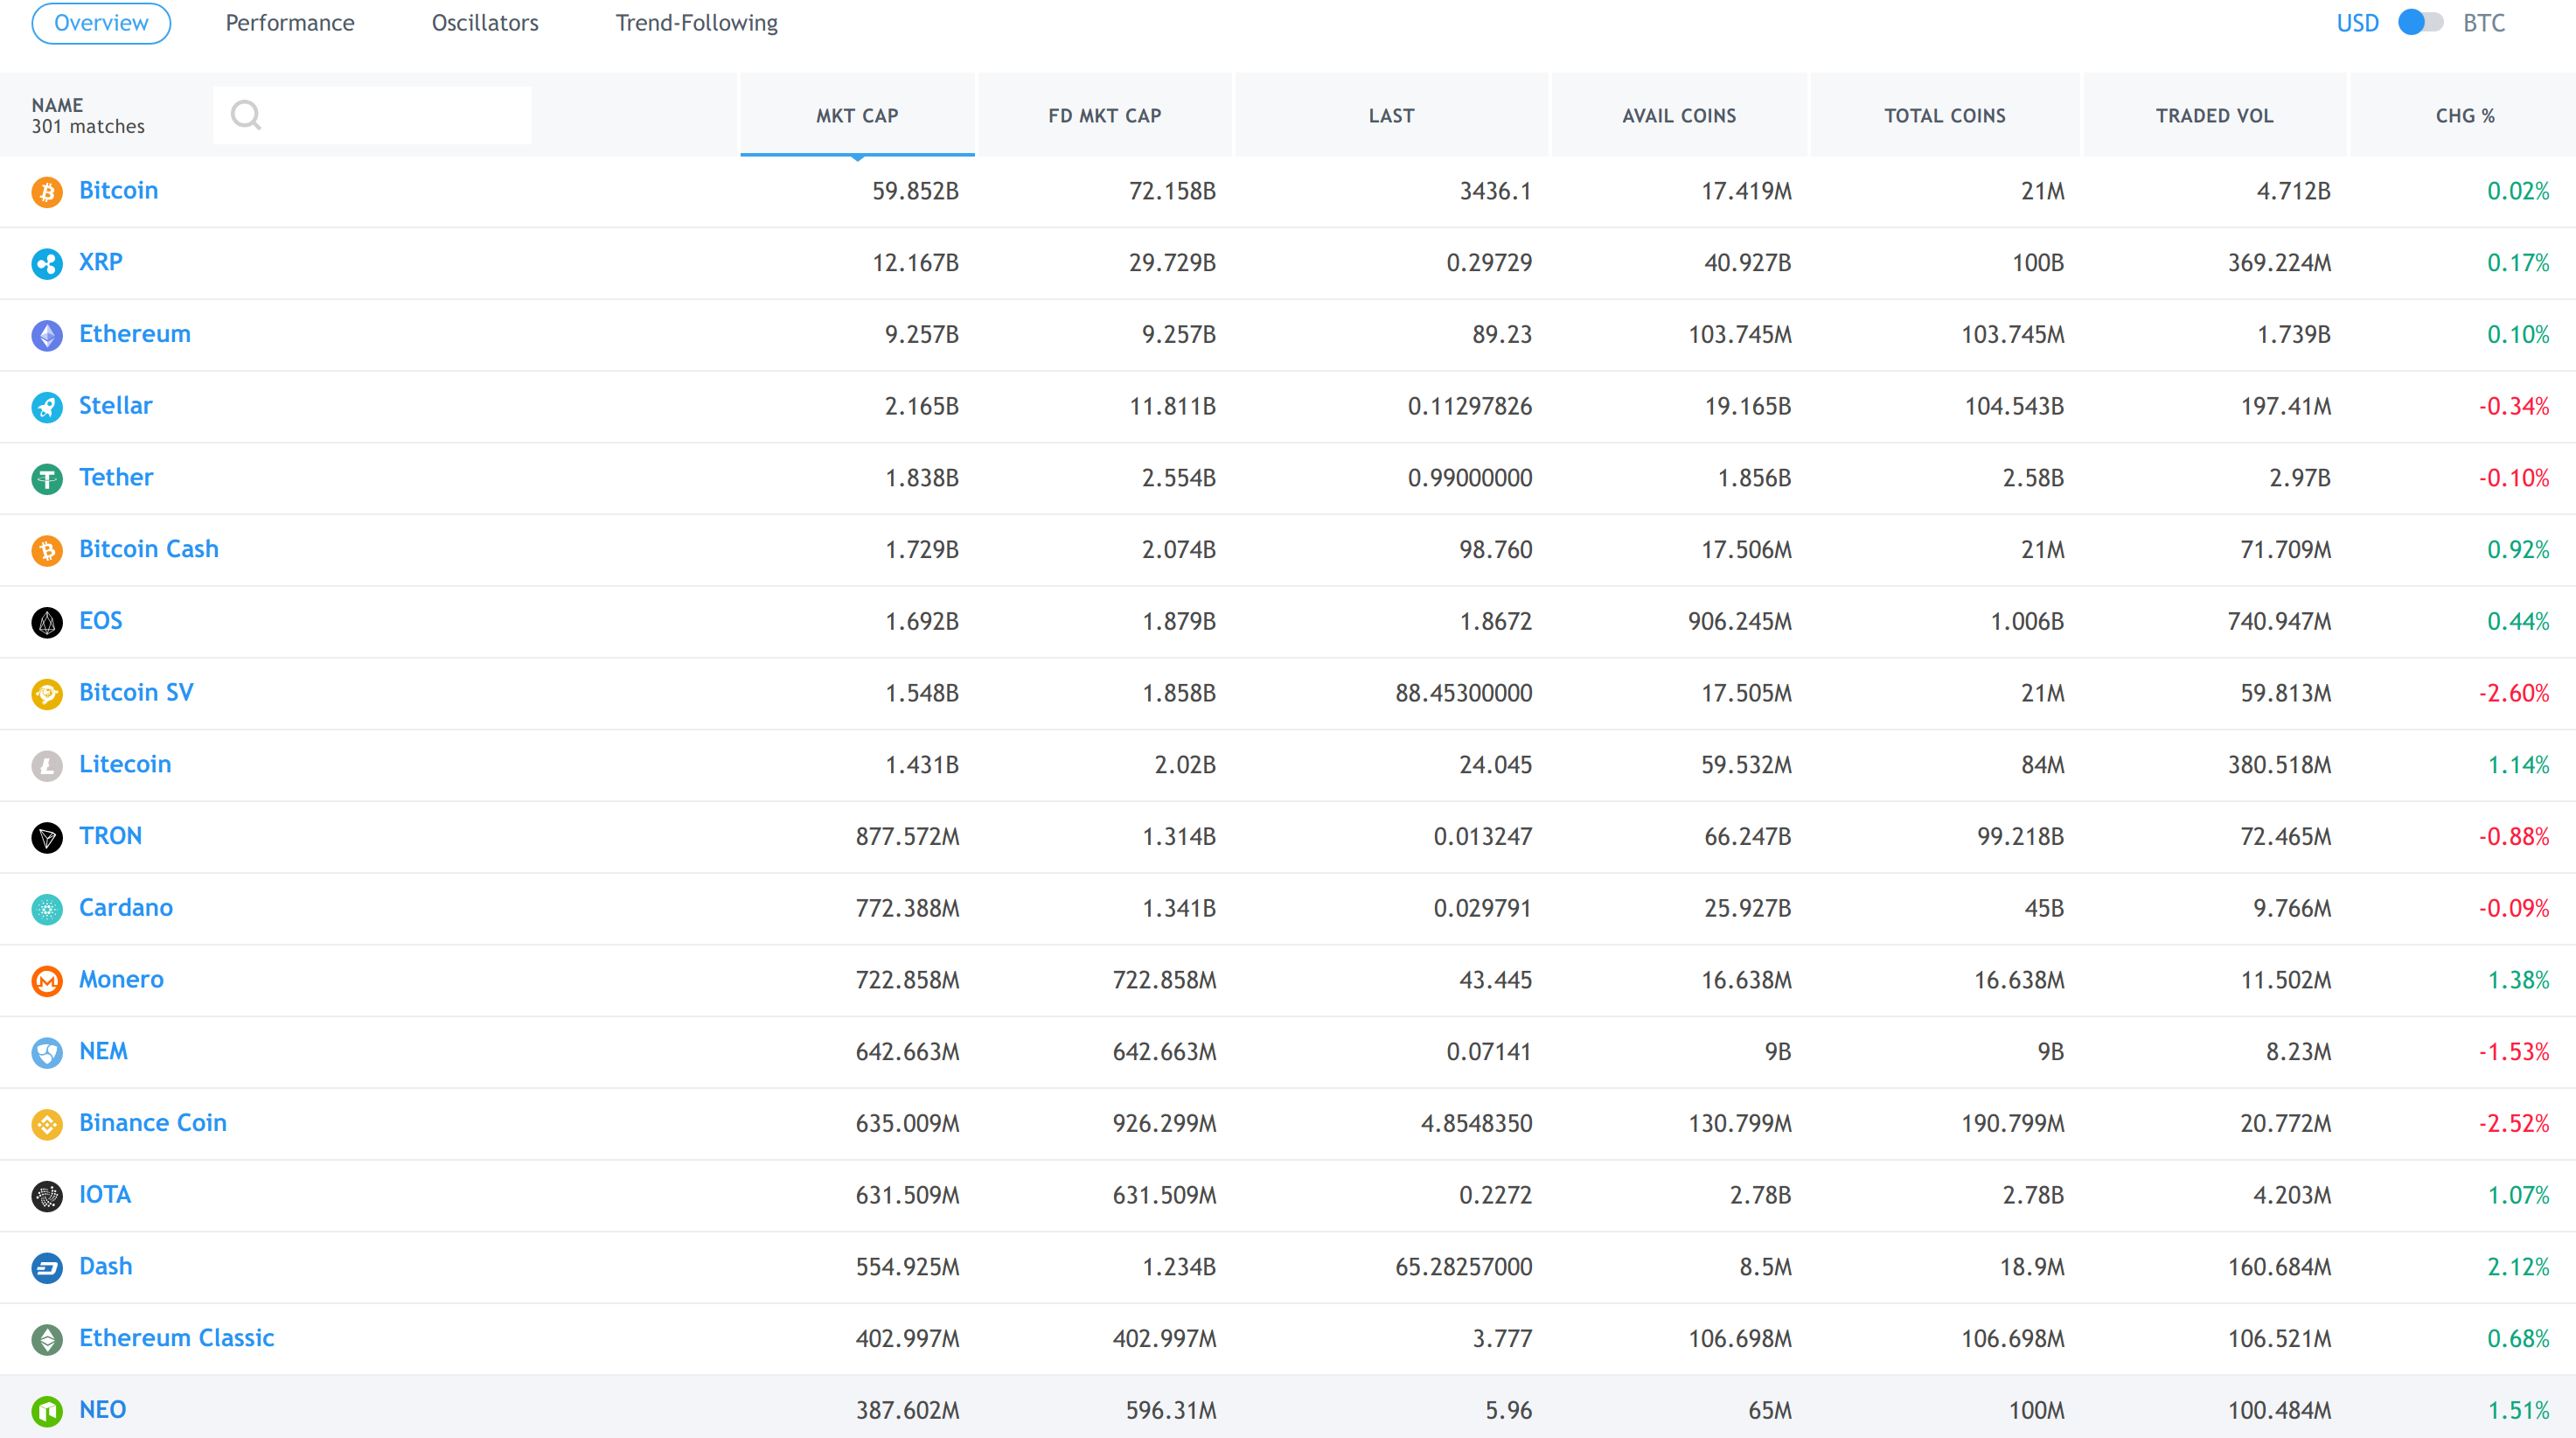
\includegraphics[width=10cm]{../pics/ethereum/coinslist-2018}
	\end{figure}
}

